% Midterm defense — EURECOM Spring 2026
% Compile: xelatex midterm_defense.tex (run twice for the table of contents)
\documentclass[aspectratio=169,11pt]{beamer}

\usetheme{metropolis}
\metroset{block=fill, sectionpage=progressbar, numbering=fraction}

\usepackage{amsmath,amssymb,bm}
\usepackage{booktabs}
\usepackage{tikz}
\usetikzlibrary{arrows.meta, positioning}

% Sober accent colour (teal), consistent with the figures
\definecolor{AccentTeal}{HTML}{2A9D8F}
\definecolor{InkNavy}{HTML}{1E2761}
\definecolor{MutedGray}{HTML}{6B7280}
\setbeamercolor{frametitle}{bg=InkNavy}
\setbeamercolor{progress bar}{fg=AccentTeal}
\setbeamercolor{alerted text}{fg=AccentTeal}

\newcommand{\E}{\mathcal{E}}
\newcommand{\R}{\mathbb{R}}

\title{Can the frozen encoder of a diffusion model detect deepfakes?}
\subtitle{An encoder-only approach, benchmarked against a ResNet baseline}
\author{Loïc Huang}
\institute{EURECOM --- Semester Research Project, Spring 2026 \\ Supervisor: Alexandre Libourel}
\date{Midterm defense --- 29 May 2026}

\begin{document}

\maketitle

\begin{frame}{Outline}
  \tableofcontents
\end{frame}

% ============================================================
\section{Introduction}

\begin{frame}{Problem setting}
  \textbf{Deepfakes} are facial images synthesised or manipulated by deep
  generative models (face-swap, reenactment).

  \medskip
  The scientific difficulty is \alert{not} in-distribution accuracy but
  \alert{generalisation}: a detector trained on one manipulation method
  typically degrades sharply on a different, unseen one.

  \medskip
  \begin{itemize}
    \item Manipulation methods evolve faster than labelled datasets.
    \item A detector must capture \emph{generation traces}, not dataset-specific cues.
    \item Cross-dataset evaluation is the appropriate stress test.
  \end{itemize}
\end{frame}

\begin{frame}{Diffusion models as feature extractors}
  Latent diffusion models (LDMs) embed an image into a latent space via an
  encoder $\E$. Recent detectors exploit this:
  \begin{itemize}
    \item Wang \& Kalogeiton (ECCV 2024): classifier-free guidance residuals
          across denoising steps.
    \item Ricker et al.\ (AEROBLADE, CVPR 2024): autoencoder reconstruction error.
  \end{itemize}
  \medskip
  Both rely on the \alert{full diffusion process} --- multiple network
  evaluations per image. We ask whether a far cheaper signal already suffices.
\end{frame}

% ============================================================
\section{Problem statement}

\begin{frame}{Research question}
  \begin{block}{Hypothesis}
    The latent representation produced by a \alert{frozen} LDM encoder,
    taken \alert{alone} --- no diffusion, no fine-tuning --- is sufficient
    to discriminate real from manipulated faces.
  \end{block}

  \medskip
  We assess the hypothesis through a \textbf{controlled comparison} against
  a standard frozen feature extractor (ResNet-50):
  \begin{itemize}
    \item identical classifier head, data and protocol;
    \item only the feature extractor changes;
    \item \alert{the backbone is frozen in all cases} (project constraint).
  \end{itemize}
\end{frame}

% ============================================================
\section{Method}

\begin{frame}{Pipeline}
  \begin{center}
  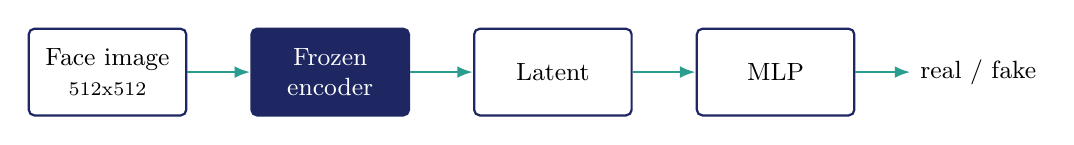
\begin{tikzpicture}[
      node distance=8mm,
      box/.style={draw=InkNavy, line width=0.8pt, rounded corners=2pt,
                  minimum height=11mm, minimum width=20mm, align=center, font=\small},
      frozen/.style={box, fill=InkNavy, text=white},
      arr/.style={-{Latex[length=2mm]}, line width=1pt, draw=AccentTeal}]
    \node[box] (img) {Face image\\\scriptsize 512x512};
    \node[frozen, right=of img] (enc) {Frozen\\encoder};
    \node[box, right=of enc] (z) {Latent};
    \node[box, right=of z] (mlp) {MLP};
    \node[right=7mm of mlp, font=\small] (out) {real / fake};
    \draw[arr] (img) -- (enc);
    \draw[arr] (enc) -- (z);
    \draw[arr] (z) -- (mlp);
    \draw[arr] (mlp) -- (out);
  \end{tikzpicture}
  \end{center}
  \medskip
  Only the MLP is trained. The extractor is frozen, so latents are
  \alert{pre-computed once} and cached --- training reduces to fitting a small
  MLP on fixed feature vectors.
\end{frame}

\begin{frame}{Two frozen feature extractors}
  \begin{columns}[T]
    \begin{column}{0.5\textwidth}
      \begin{block}{LDM encoder}
        Stable Diffusion 1.4 VAE encoder \\
        (Wang \& Kalogeiton source). \\[2mm]
        latent 4 x 64 x 64 \\
        $\Rightarrow$ 16\,384 features
      \end{block}
    \end{column}
    \begin{column}{0.5\textwidth}
      \begin{block}{ResNet-50 (baseline)}
        ImageNet-pretrained. \\
        Global-average-pooled features \\
        (layer before the head). \\[2mm]
        $\Rightarrow$ 2\,048 features
      \end{block}
    \end{column}
  \end{columns}
  \medskip
  \textbf{Identical} downstream 3-layer MLP with ReLU activations and
  dropout $0.3$. The only variable is the extractor.
\end{frame}

% ============================================================
\section{Experimental setup}

\begin{frame}{Datasets and protocol}
  \begin{itemize}
    \item \textbf{In-domain (train/val/test):} FaceForensics++, c23
          compression, pre-cropped faces. \alert{Manipulation used:
          DeepFakes} (one of the four FF++ manipulations available, the
          other three are reserved for future work).
    \item \textbf{Cross-dataset (test only):} Celeb-DF-v2 --- never seen
          during training; measures generalisation.
    \item \textbf{Splits:} official Rössler 2019 splits ---
          \alert{identity-disjoint}, preventing identity leakage that would
          inflate the score.
    \item \textbf{Sampling:} 5 frames per video. \textbf{Metric:} AUC, with
          a 95\% video-level bootstrap confidence interval.
  \end{itemize}
  \medskip
  \centering
  \footnotesize
  7190 train \;/\; 1397 val \;/\; 1400 FF++ test \;/\; 2590 Celeb-DF test.
\end{frame}

% ============================================================
\section{Results}

\begin{frame}{Main comparison (both extractors frozen)}
  \begin{columns}[T]
    \begin{column}{0.46\textwidth}
      \centering
      \renewcommand{\arraystretch}{1.3}
      \begin{tabular}{lcc}
        \toprule
        \textbf{Extractor} & \textbf{FF++} & \textbf{Celeb-DF} \\
        \midrule
        LDM encoder & \textcolor{AccentTeal}{\textbf{0.87}} & 0.52 \\
        ResNet-50   & 0.78 & 0.54 \\
        \bottomrule
      \end{tabular}

      \medskip
      \footnotesize AUC with 95\% video-level bootstrap CI. In-domain, the
      diffusion encoder exceeds the ResNet baseline; cross-dataset, both
      collapse toward chance ($0.5$).
    \end{column}
    \begin{column}{0.54\textwidth}
      \centering
      \IfFileExists{../results/auc_bars_ci.png}{%
        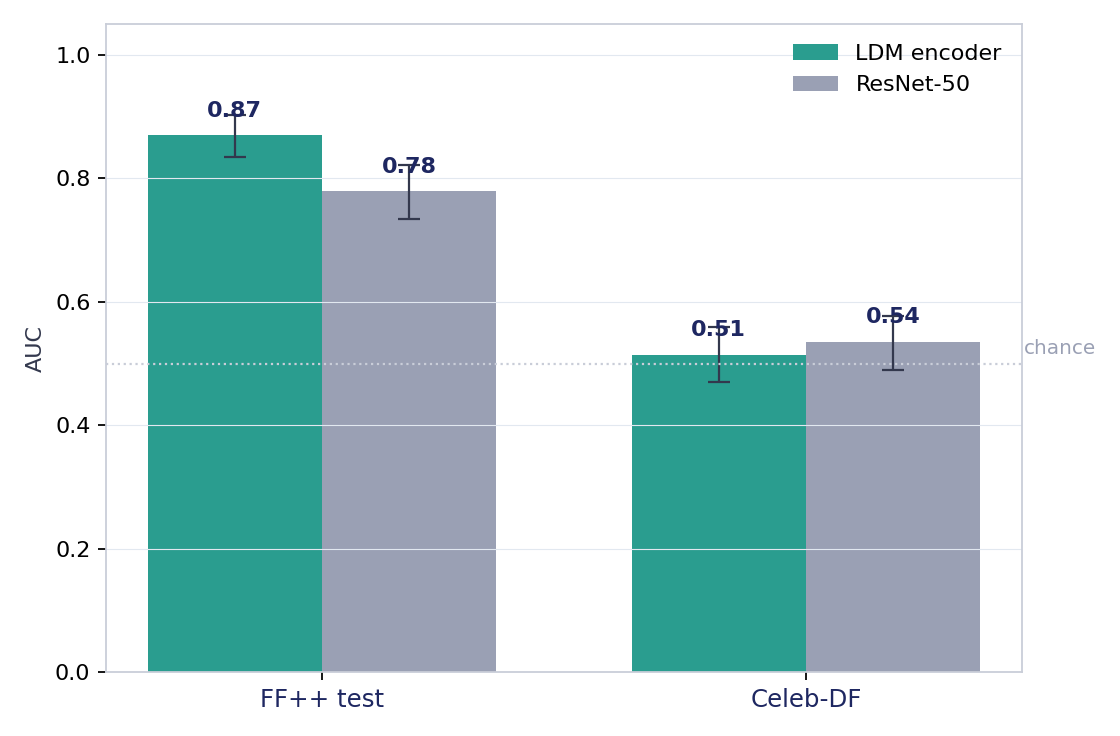
\includegraphics[width=\linewidth]{../results/auc_bars_ci.png}%
      }{%
        \vspace{1.5cm}\textit{\small AUC bar chart with 95\% CI\\
        (generated by \texttt{make\_figures.py})}\vspace{1.5cm}%
      }
    \end{column}
  \end{columns}
\end{frame}

\begin{frame}{ROC analysis}
  \centering
  \IfFileExists{../results/roc_curves.png}{%
    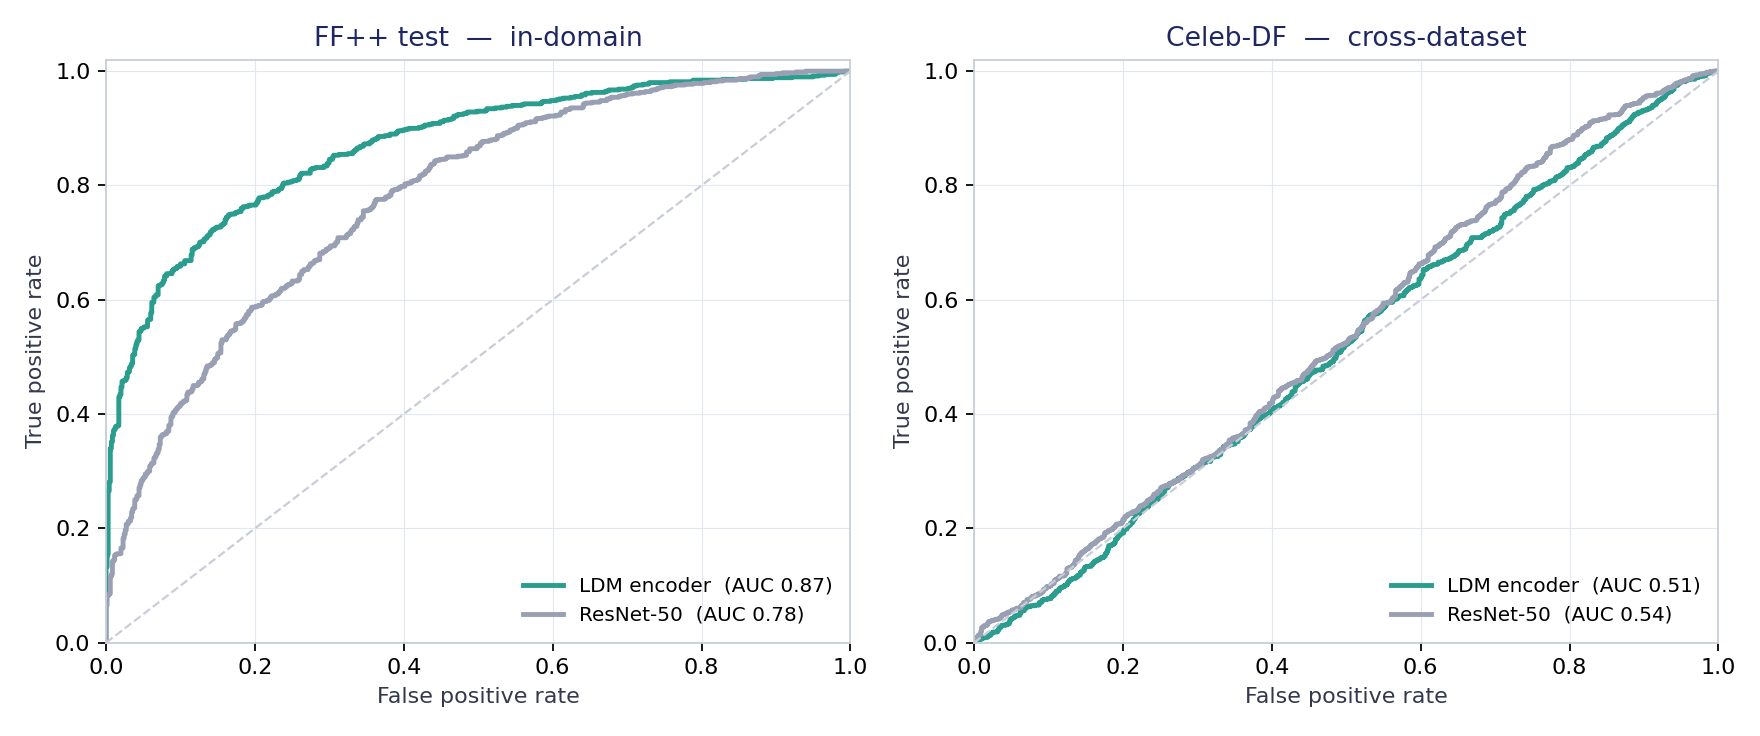
\includegraphics[width=0.95\textwidth]{../results/roc_curves.png}%
  }{%
    \vspace{2cm}\textit{ROC curves for FF++ (in-domain) and Celeb-DF
    (cross-dataset), LDM vs ResNet\\
    (generated by \texttt{make\_figures.py})}\vspace{2cm}%
  }
\end{frame}

\begin{frame}{In-domain finding}
  \begin{block}{Result}
    At an equal frozen setup and an identical classifier, the diffusion
    encoder extracts \alert{more discriminative} features than a standard
    ResNet: AUC 0.87 [0.835, 0.903] versus 0.78 [0.734, 0.822] on FF++.
  \end{block}
  \medskip
  \begin{itemize}
    \item The 95\% confidence intervals are \alert{disjoint}
          (0.835 > 0.822): the in-domain superiority is statistically
          significant.
    \item Supports the hypothesis: the encoder-only representation is
          \emph{not} too weak.
  \end{itemize}
\end{frame}

\begin{frame}{Generalisation gap}
  Cross-dataset, both extractors fall close to chance: LDM
  0.52 [0.471, 0.559], ResNet 0.54 [0.490, 0.577]. Both confidence
  intervals contain 0.5 and overlap --- statistically indistinguishable
  from chance, and from each other.

  \medskip
  \begin{block}{Diagnostic}
    A linear probe trained \emph{directly} on Celeb-DF latents reaches an
    AUC of about 0.74: the discriminative signal \alert{exists}. The
    FF++-trained classifier simply fails to transfer.
  \end{block}
  \medskip
  $\Rightarrow$ This is a \textbf{domain gap}, common to both extractors --- a
  limitation of the frozen, single-manipulation setup, not a flaw specific to
  the diffusion encoder.
\end{frame}

% ============================================================
\section{Discussion and next steps}

\begin{frame}{Next steps (frozen-backbone compatible)}
  \begin{enumerate}
    \item \textbf{Improve the MLP head} --- explore deeper or wider
          variants, dimensionality reduction of the latent (pooling),
          stronger regularisation, hyper-parameter tuning. The bottleneck
          appears to be the classifier capacity, not the extractor.
    \item \textbf{Train on the other FF++ manipulations} --- currently
          only DeepFakes is used; adding Face2Face, FaceSwap and
          NeuralTextures should expose the head to more diverse generation
          traces and improve cross-method generalisation.
  \end{enumerate}
  \medskip
  Both steps preserve the frozen-backbone constraint: only the head and the
  training distribution change.
\end{frame}

\begin{frame}{Conclusion}
  \begin{itemize}
    \item The frozen LDM encoder is a \alert{promising} feature extractor:
          it outperforms a frozen ResNet in-domain (0.87 vs 0.78,
          confidence intervals disjoint).
    \item Cross-dataset generalisation is the \alert{open challenge}, and is
          common to both extractors --- a characterised domain gap.
    \item A clear, constraint-compatible path forward: a stronger
          classifier head and more manipulation diversity, backbone kept
          frozen.
  \end{itemize}
\end{frame}

\begin{frame}[standout]
  Thank you --- questions welcome.
\end{frame}

\appendix

\begin{frame}{References}
  \footnotesize
  \begin{enumerate}
    \item Yan et al. \emph{DeepfakeBench}, NeurIPS 2023.
    \item Wang \& Kalogeiton. \emph{Exposing the Fakes}, ECCV 2024.
    \item Ricker et al. \emph{AEROBLADE}, CVPR 2024.
    \item Rössler et al. \emph{FaceForensics++}, ICCV 2019.
    \item Li et al. \emph{Celeb-DF}, CVPR 2020.
  \end{enumerate}
\end{frame}

\end{document}
